\documentclass[12pt, twoside]{article}
\usepackage[francais]{babel}
\usepackage[T1]{fontenc}
\usepackage[latin1]{inputenc}
\usepackage[left=7mm, right=7mm, top=5mm, bottom=5mm]{geometry}
\usepackage{float}
\usepackage{graphicx}
\usepackage{array}
\usepackage{multirow}
\usepackage{amsmath,amssymb,mathrsfs}
\usepackage{soul}
\usepackage{textcomp}
\usepackage{eurosym}
 \usepackage{variations}
\usepackage{tabvar}


\pagestyle{empty}

\begin{document}

\begin{flushleft}
NOM PRENOM: \ldots \ldots \ldots \ldots \ldots \ldots \ldots \ldots \ldots
\ldots \ldots
\end{flushleft}


\section*{\center{Devoir maison 2}}


\bigskip





\fbox{

\begin{minipage}{18cm}
\textit{Devoir � rendre pour le \textbf{\ldots \ldots \ldots \ldots \ldots
 \ldots d�cembre}.
Les exercices 1 et 3 sont � faire sur la photocopie. L'exercice 2 se fait sur une
\textbf{feuille blanche} (� coller sur votre feuille de classeur pr�par�e).}
\end{minipage}
}

\bigskip


\ul{Exercice 1}: (\textbf{4 points}) 


\begin{center}
	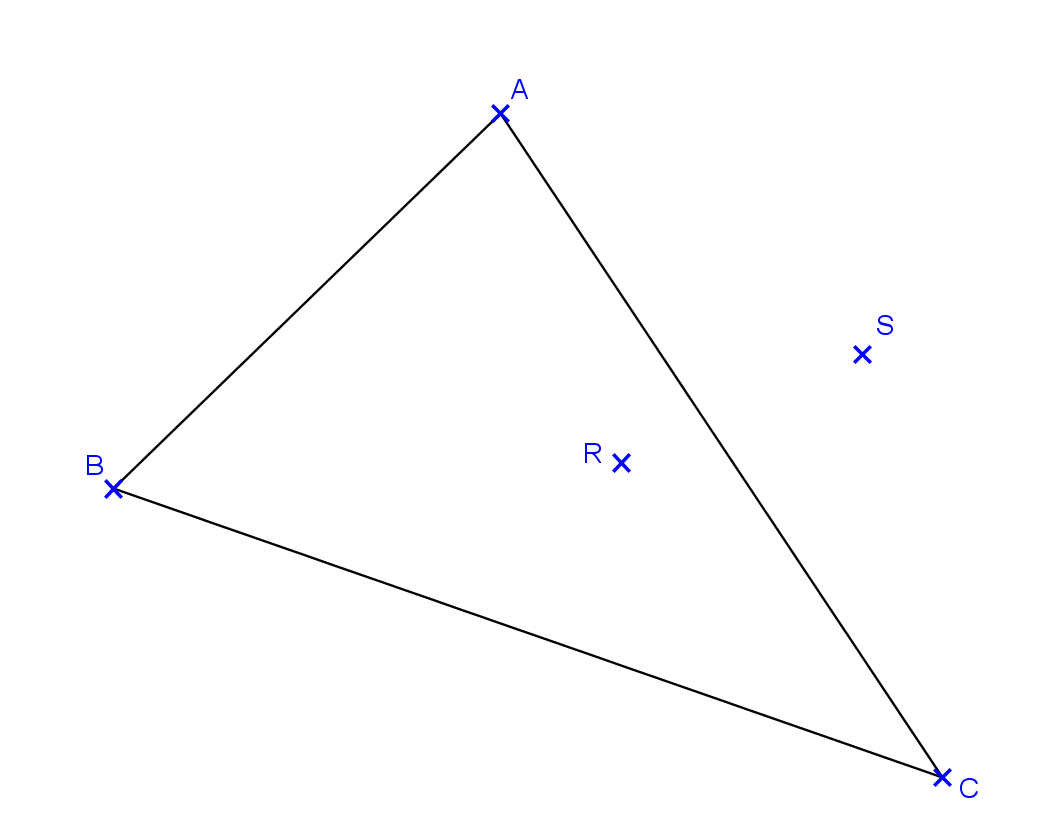
\includegraphics[width=11cm]{images/exo1.png}
\end{center}

Sur la figure ci-dessus, tracer � l'aide d'une �querre et (ou) d'une r�gle gradu�e : 
\begin{enumerate}
  \item en bleu la parall�le � la droite $(AB)$ passant par le point $R$,
  \item en rouge la perpendiculaire � la droite $(AC)$ passant par le point $R$,
  \item en vert la parall�le � la droite $(BC)$ passant par le point $S$.
\end{enumerate} 


\bigskip


\ul{Exercice 2}: (\textbf{4,5 points})




\begin{tabular}{cc}
\begin{minipage}{13cm}
Tracer une figure (� l'aide d'une �querre et (ou) d'une r�gle gradu�e) respectant les codages et les informations
donn�s sur le sch�ma ci-contre.


\end{minipage}
& 
\begin{minipage}{5,5cm}
\begin{center}
	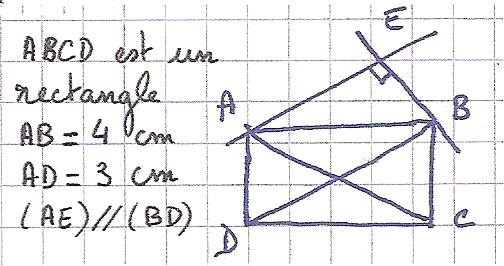
\includegraphics[width=53mm]{images/exo4.JPG}
\end{center}
\end{minipage}
\end{tabular}
\bigskip


\ul{Exercice 3}: (\textbf{2,5 points})

\begin{tabular}{cc}
\begin{minipage}{8cm}
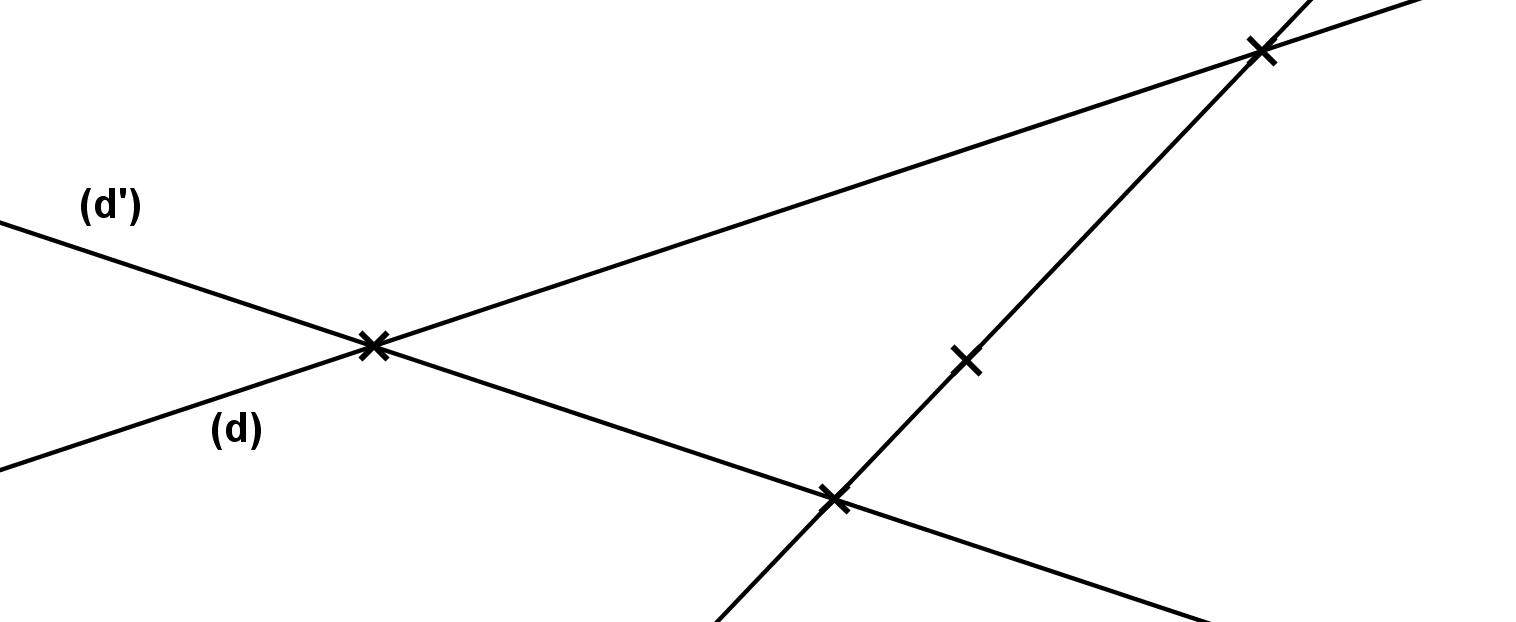
\includegraphics[width=7cm]{images/DM2_ex3.png}
\end{minipage} 
&
\begin{minipage}{10cm}
Description de la figure: 

$\bullet$ (d) et (d') sont s�cantes en B,

$\bullet A \notin (d)$ et $A \notin (d')$,

$\bullet$ (AE) coupe (d') en F.
\end{minipage}
\end{tabular}


\enskip


\begin{enumerate}
  \item Placer les points A, B, E et F de fa�on � ce que la description soit
  v�rifi�e.
  \item Compl�ter: B est le \ldots \ldots \ldots \ldots \ldots \ldots \ldots
  \ldots \ldots \ldots \ldots \ldots \ldots \ldots \ldots des droites (d) et (d').
\end{enumerate}

\pagebreak



\ul{Exercice 4}: (\textbf{4 points})

R�diger un programme de construction qui permet de r�aliser cette figure (on ne
tiendra pas compte des mesures).

\begin{center}
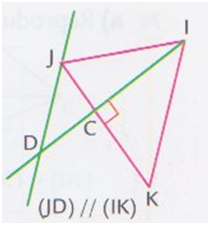
\includegraphics[width=5cm]{images/DM2_ex4.png}
\end{center}

\bigskip


\ul{Exercice 5}: (\textbf{5 points})

\begin{center}

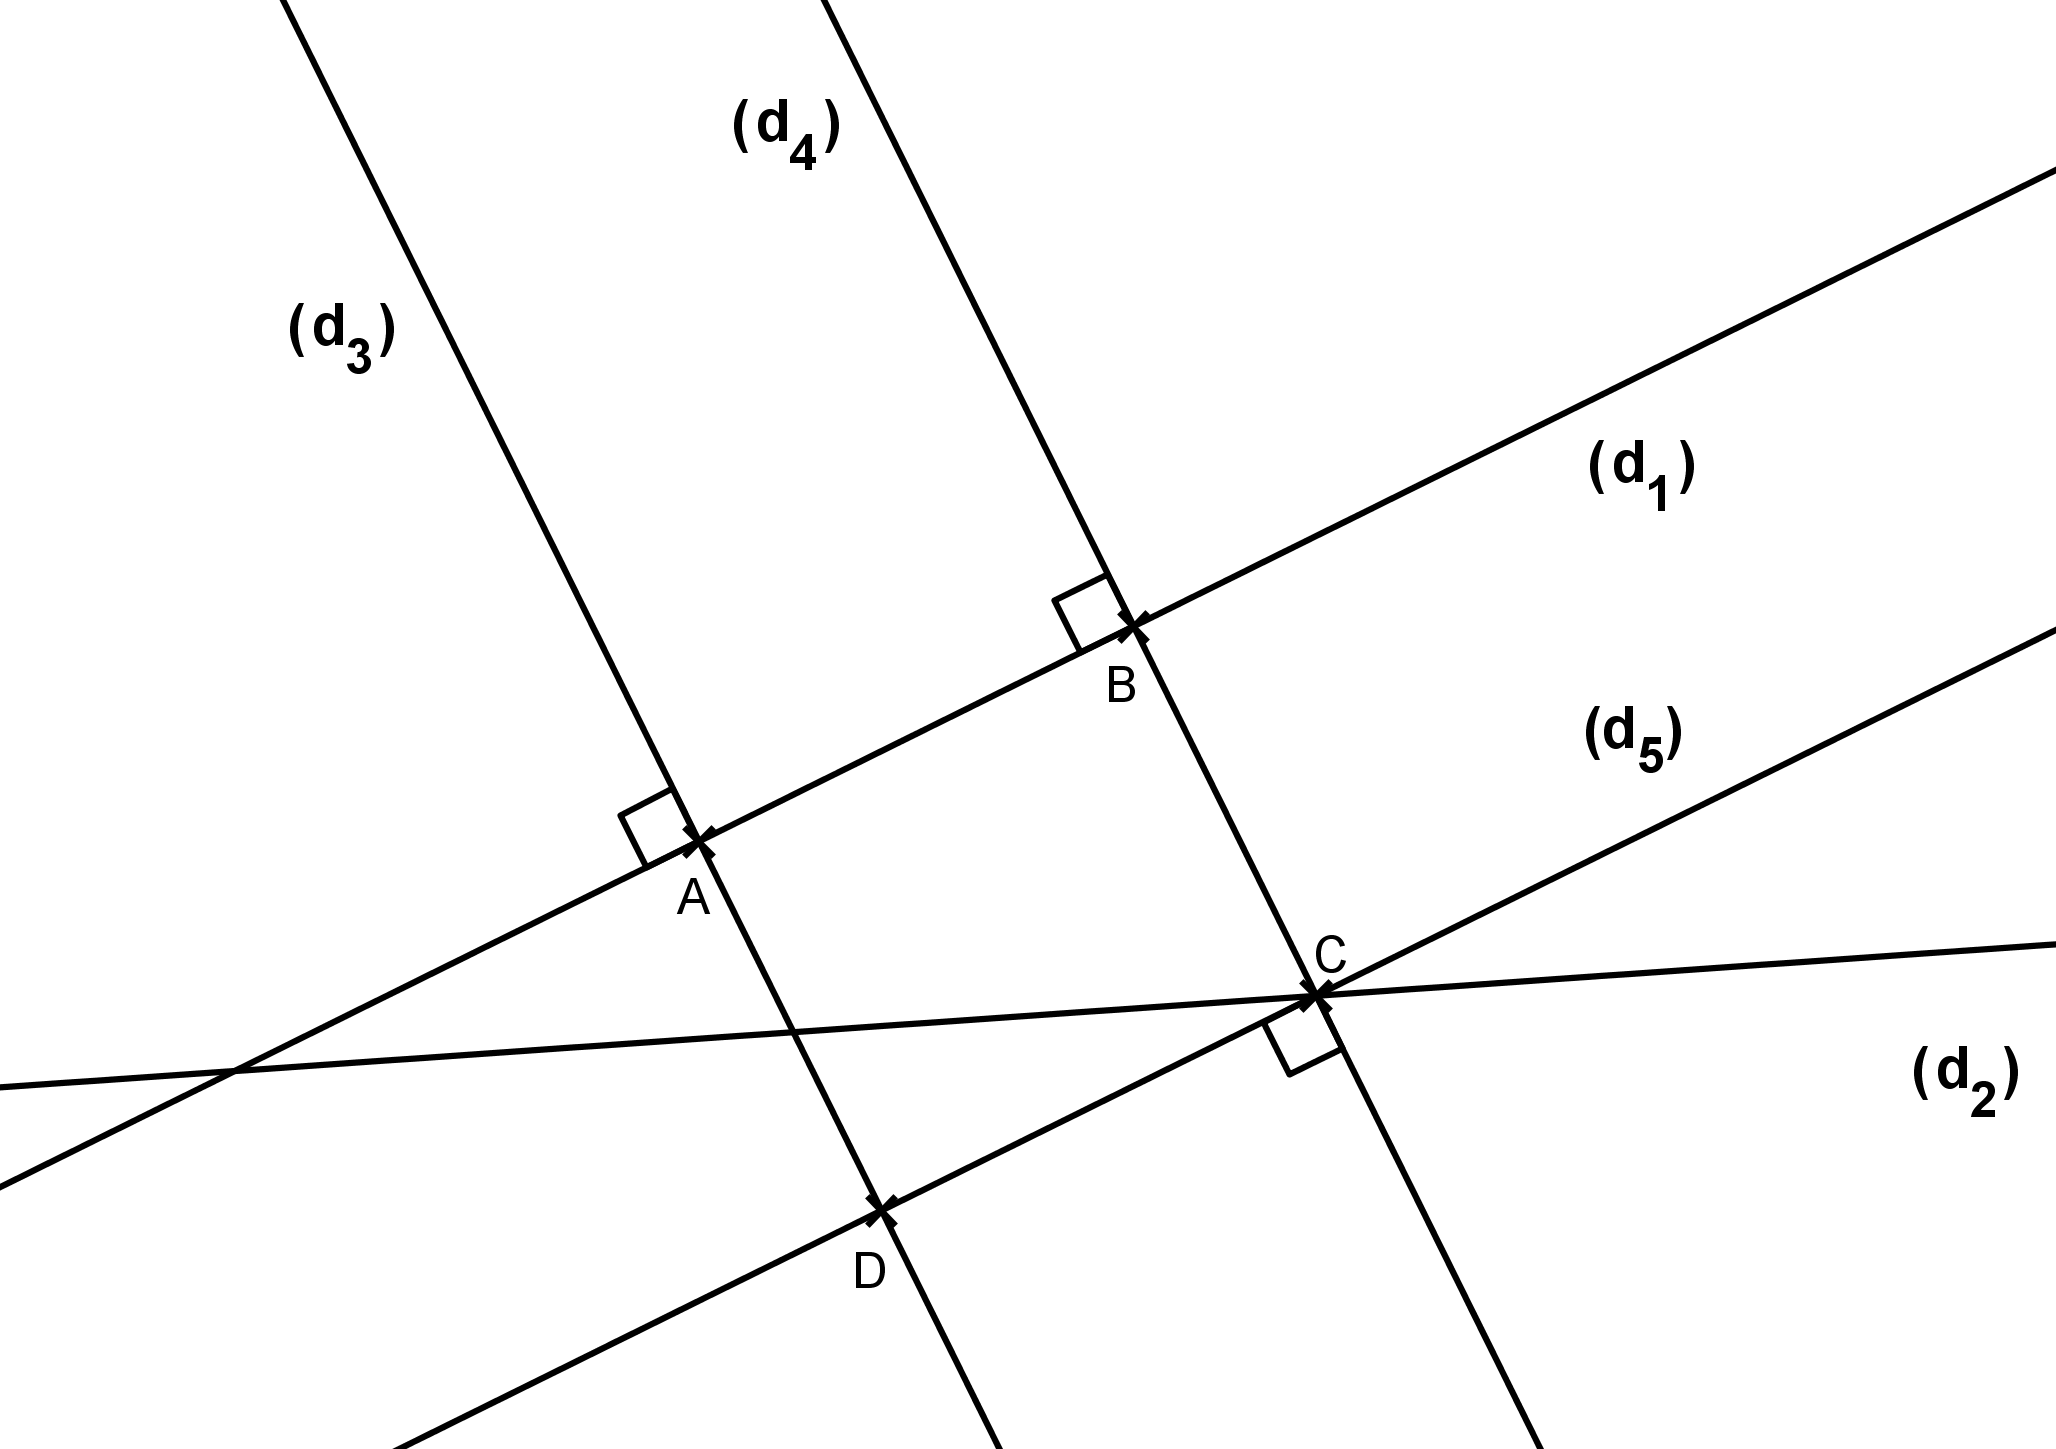
\includegraphics[width=10cm]{images/DM2_ex5.png}
\end{center}

\begin{enumerate}
  \item Donner la liste des renseignements fournis par les codages sur la
  figure ci-dessous.
  \item Recopier et compl�ter ce raisonnement:
  
  On sait que: $(d_3) \perp$ \ldots \ldots et \ldots \ldots $\perp (d_1)$.
  
  Or si deux droites sont \ldots \ldots � une m�me droite alors elles sont
  \ldots \ldots .
  
  Donc: $(d_3) \ldots (d_4)$.
  
  \item Montrer que les droites $(d_3)$ et $(d_5)$ sont perpendiculaires
  (en r�digeant comme la question 2).
  \item Quelle est la nature du quadrilat�re ABCD? Justifier votre r�ponse.
\end{enumerate}
\end{document}
